\section{Results}

When testing the developed Simulink model and Matlab script we were able to get everything generally working. We were able to capture the image (Fig \ref{fig:cameraPose}), extract the tag poses, transform them into the base frame, and then pick-up (Fig \ref{fig:PickPose}) and dropoff the object (Fig \ref{fig:DropPose}) from those locations. This all went relatively smoothly with only some minor fine-tuning of the location of the camera relative to the wrist since the initial location was an estimate with rulers as there was no official documentation on the location of the camera relative to the wrist that we could find. Once this was tuned the model worked pretty well with the added restriction of avoiding placing the tags at the extreme edges of the image as that could cause errors in the pose extraction. The locations of the tags in Figure \ref{Fig:QARM_CamPic} are pretty close to as far left and right as we found work while they could be a bit further and closer while still extracting the pose correctly and being able to reach it with the arm.

\begin{figure}[htb]
\centering
\label{fig:cameraPose}
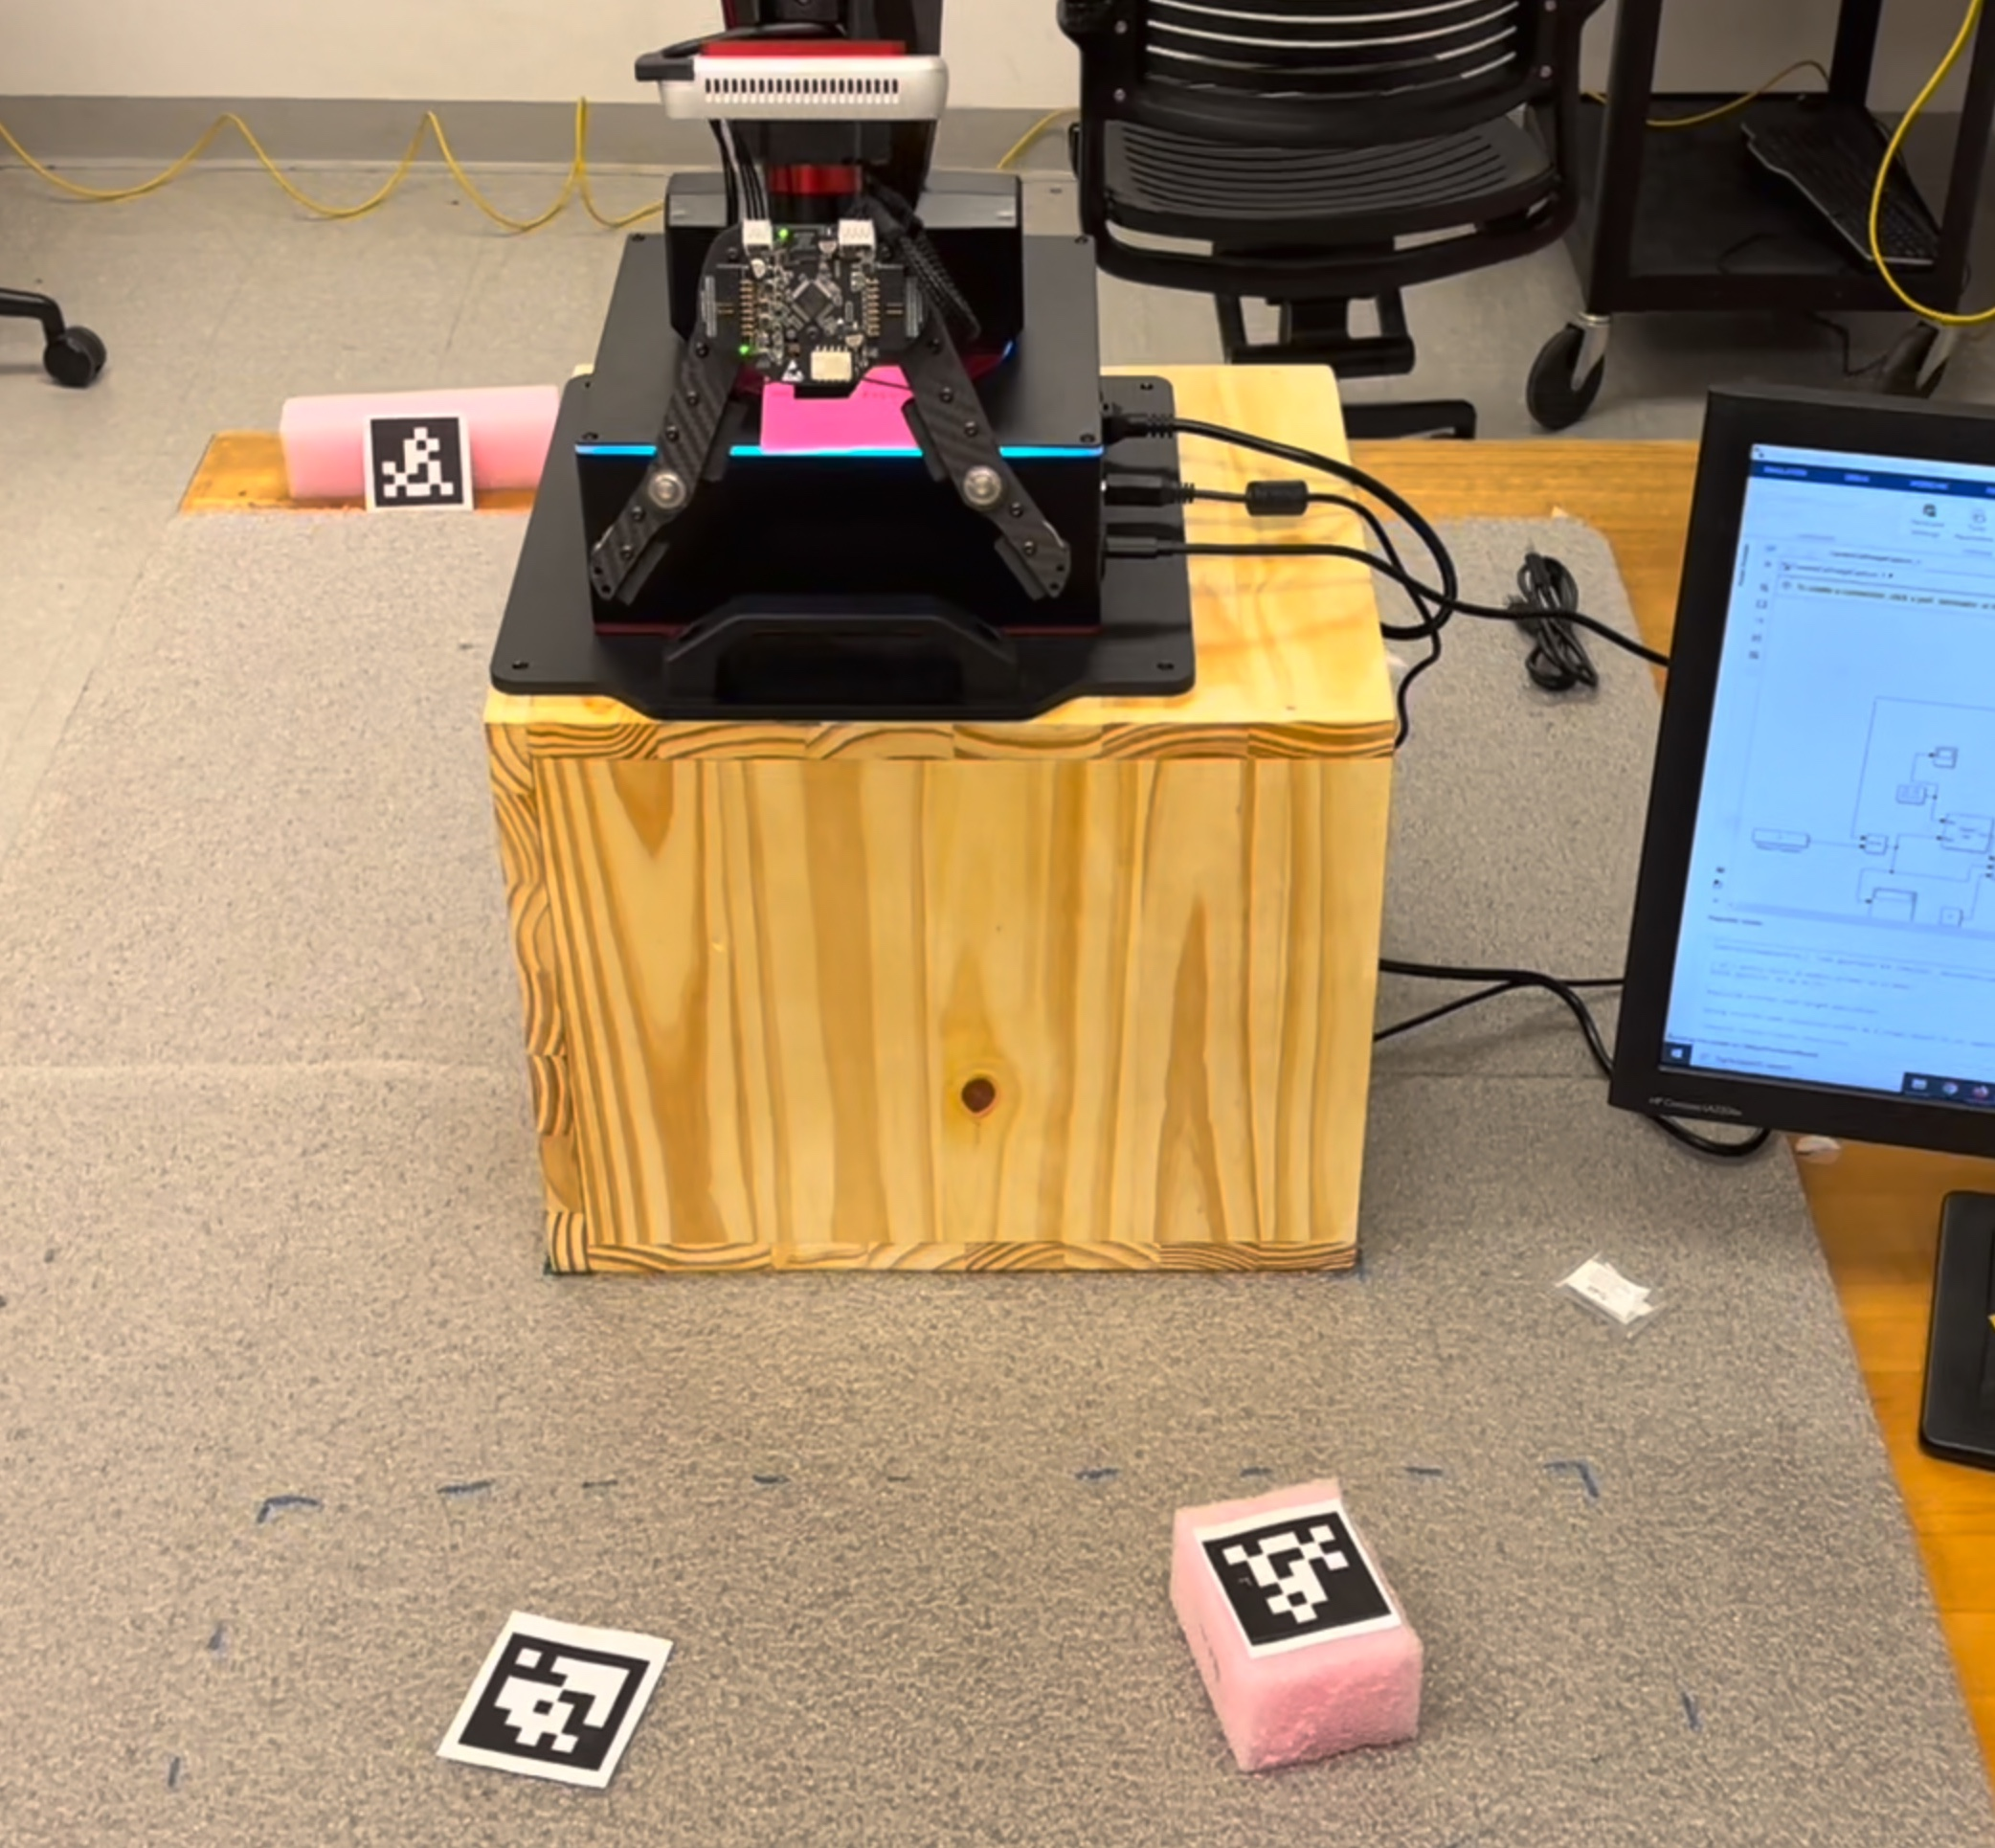
\includegraphics[width=7cm]{Figures/CamPic.jpeg}
\caption{Taking the picture for extracting the tag poses}
\centering
\end{figure}

\begin{figure}[htb]
\centering
\label{fig:PickPose}
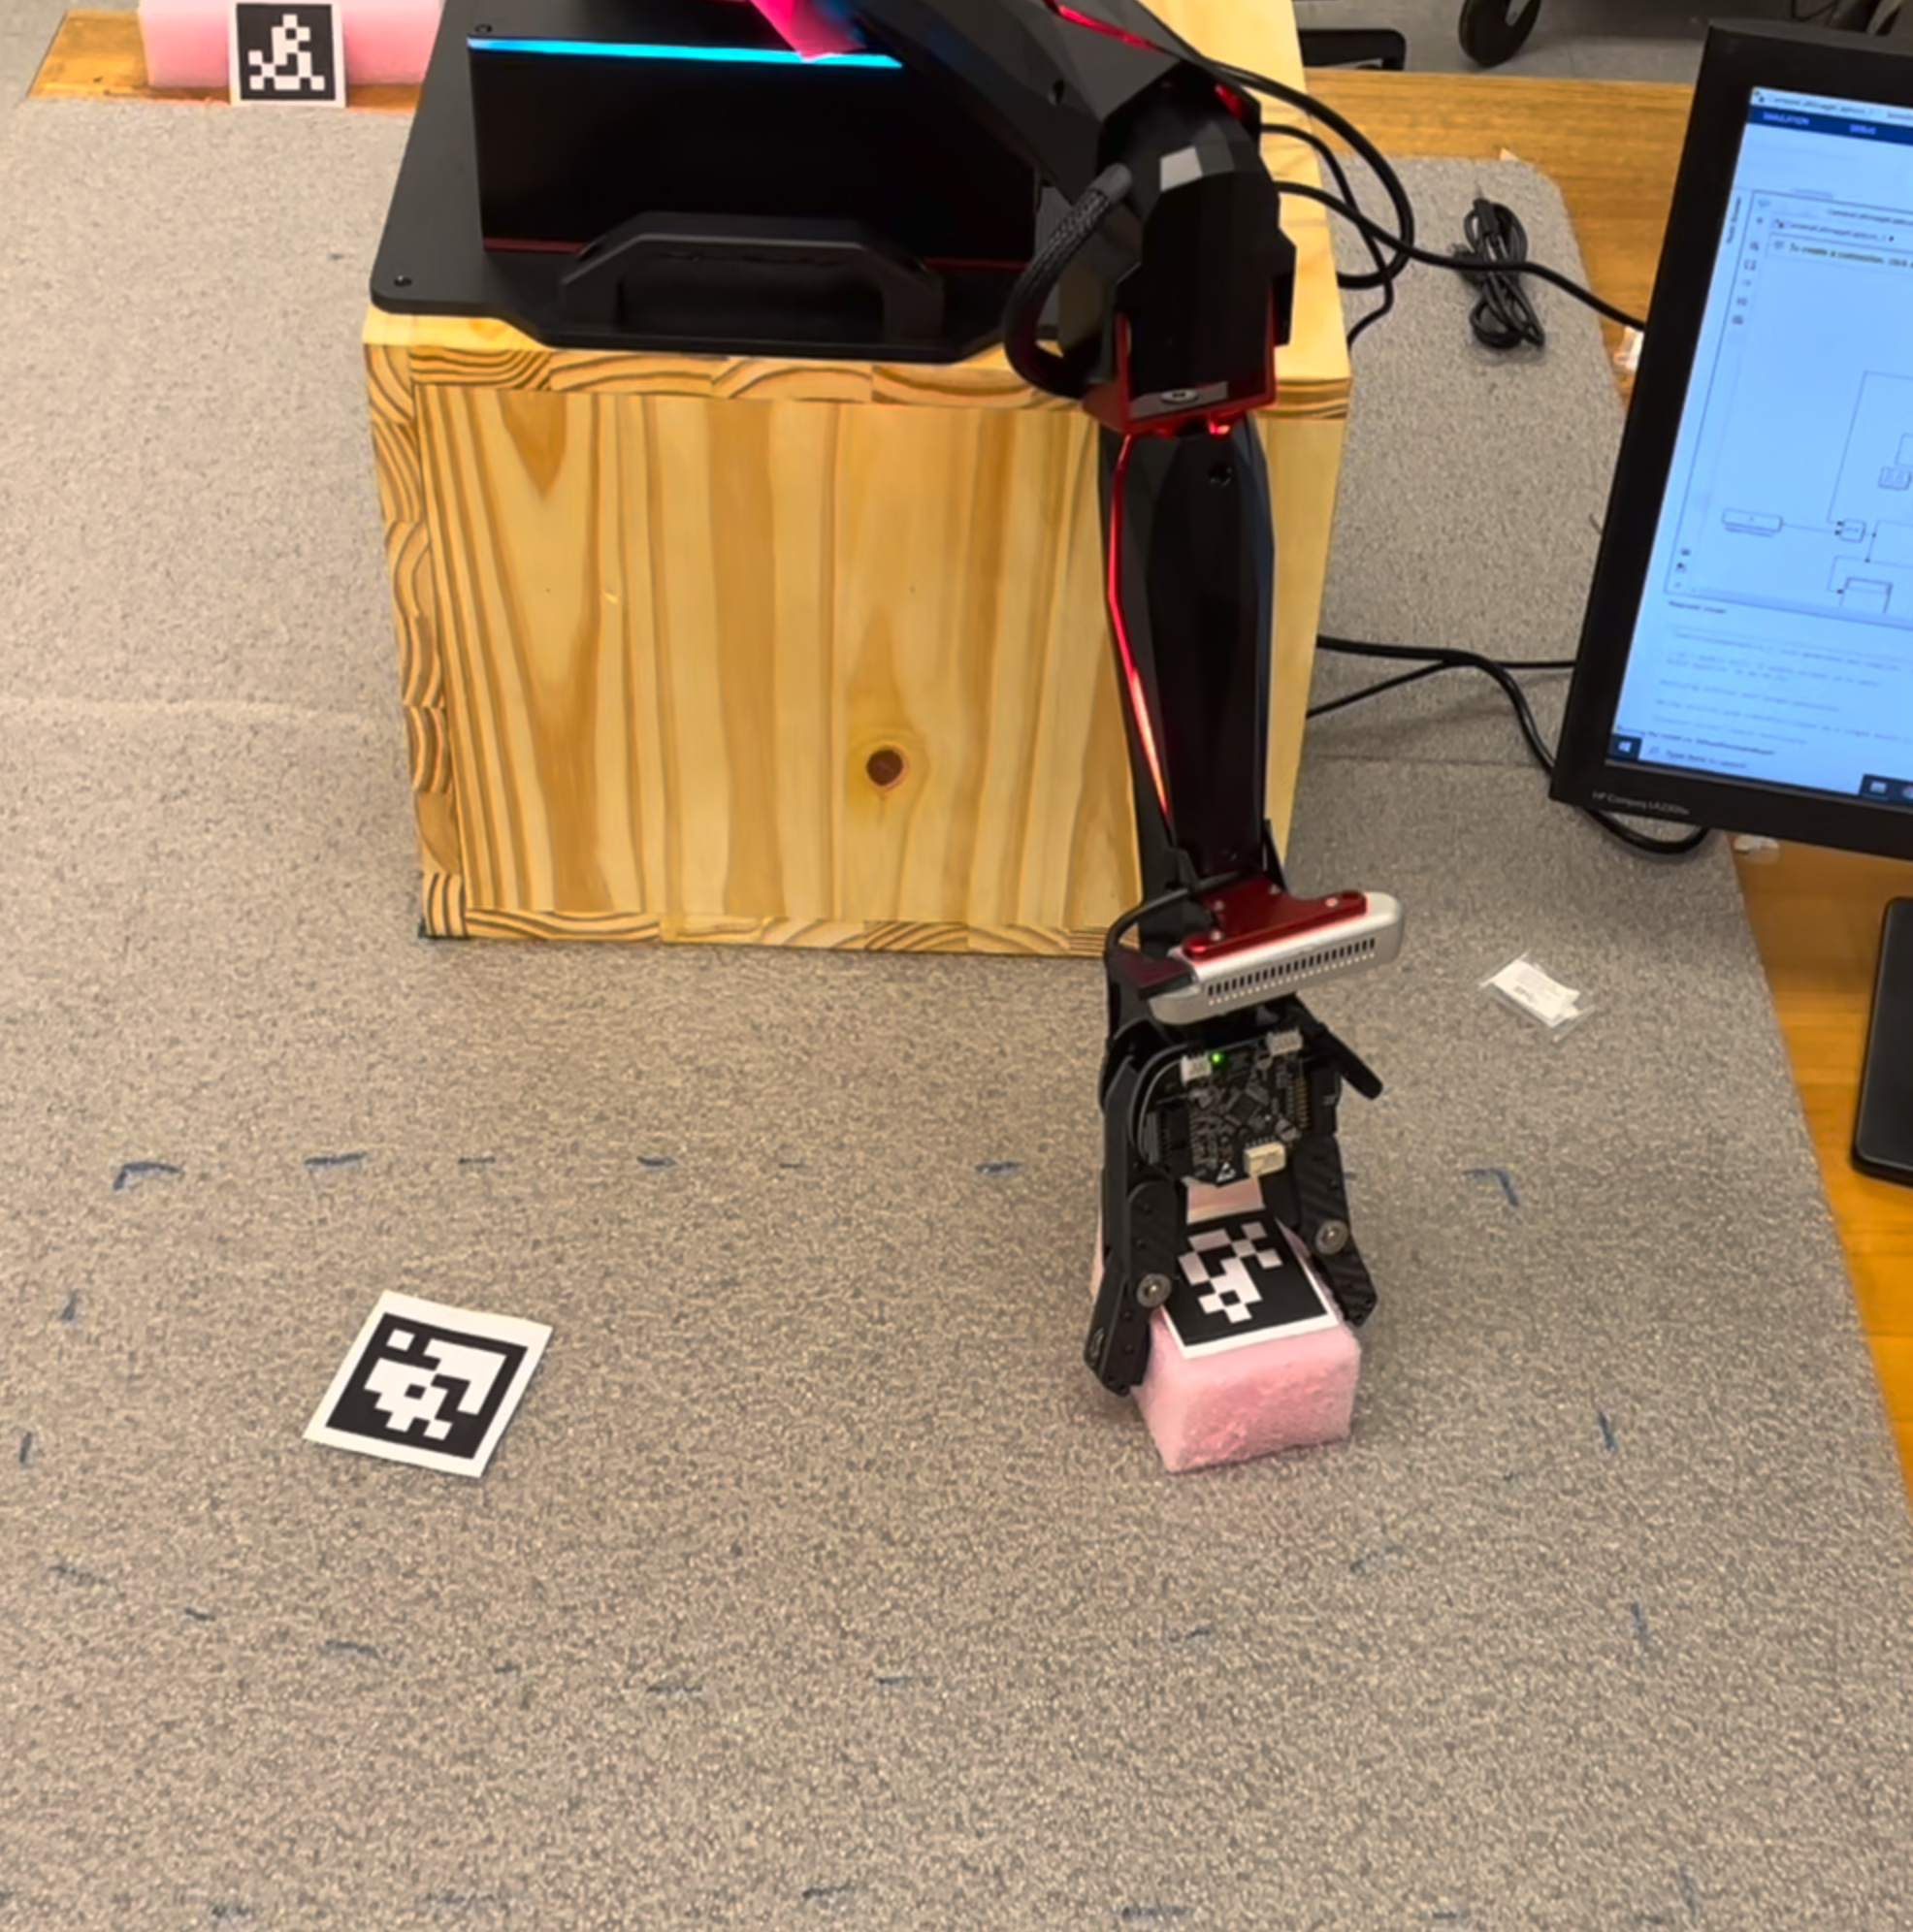
\includegraphics[width=7cm]{Figures/PickObject.jpeg}
\caption{Picking up the object}
\centering
\end{figure}

\begin{figure}[htb]
\centering
\label{fig:DropPose}
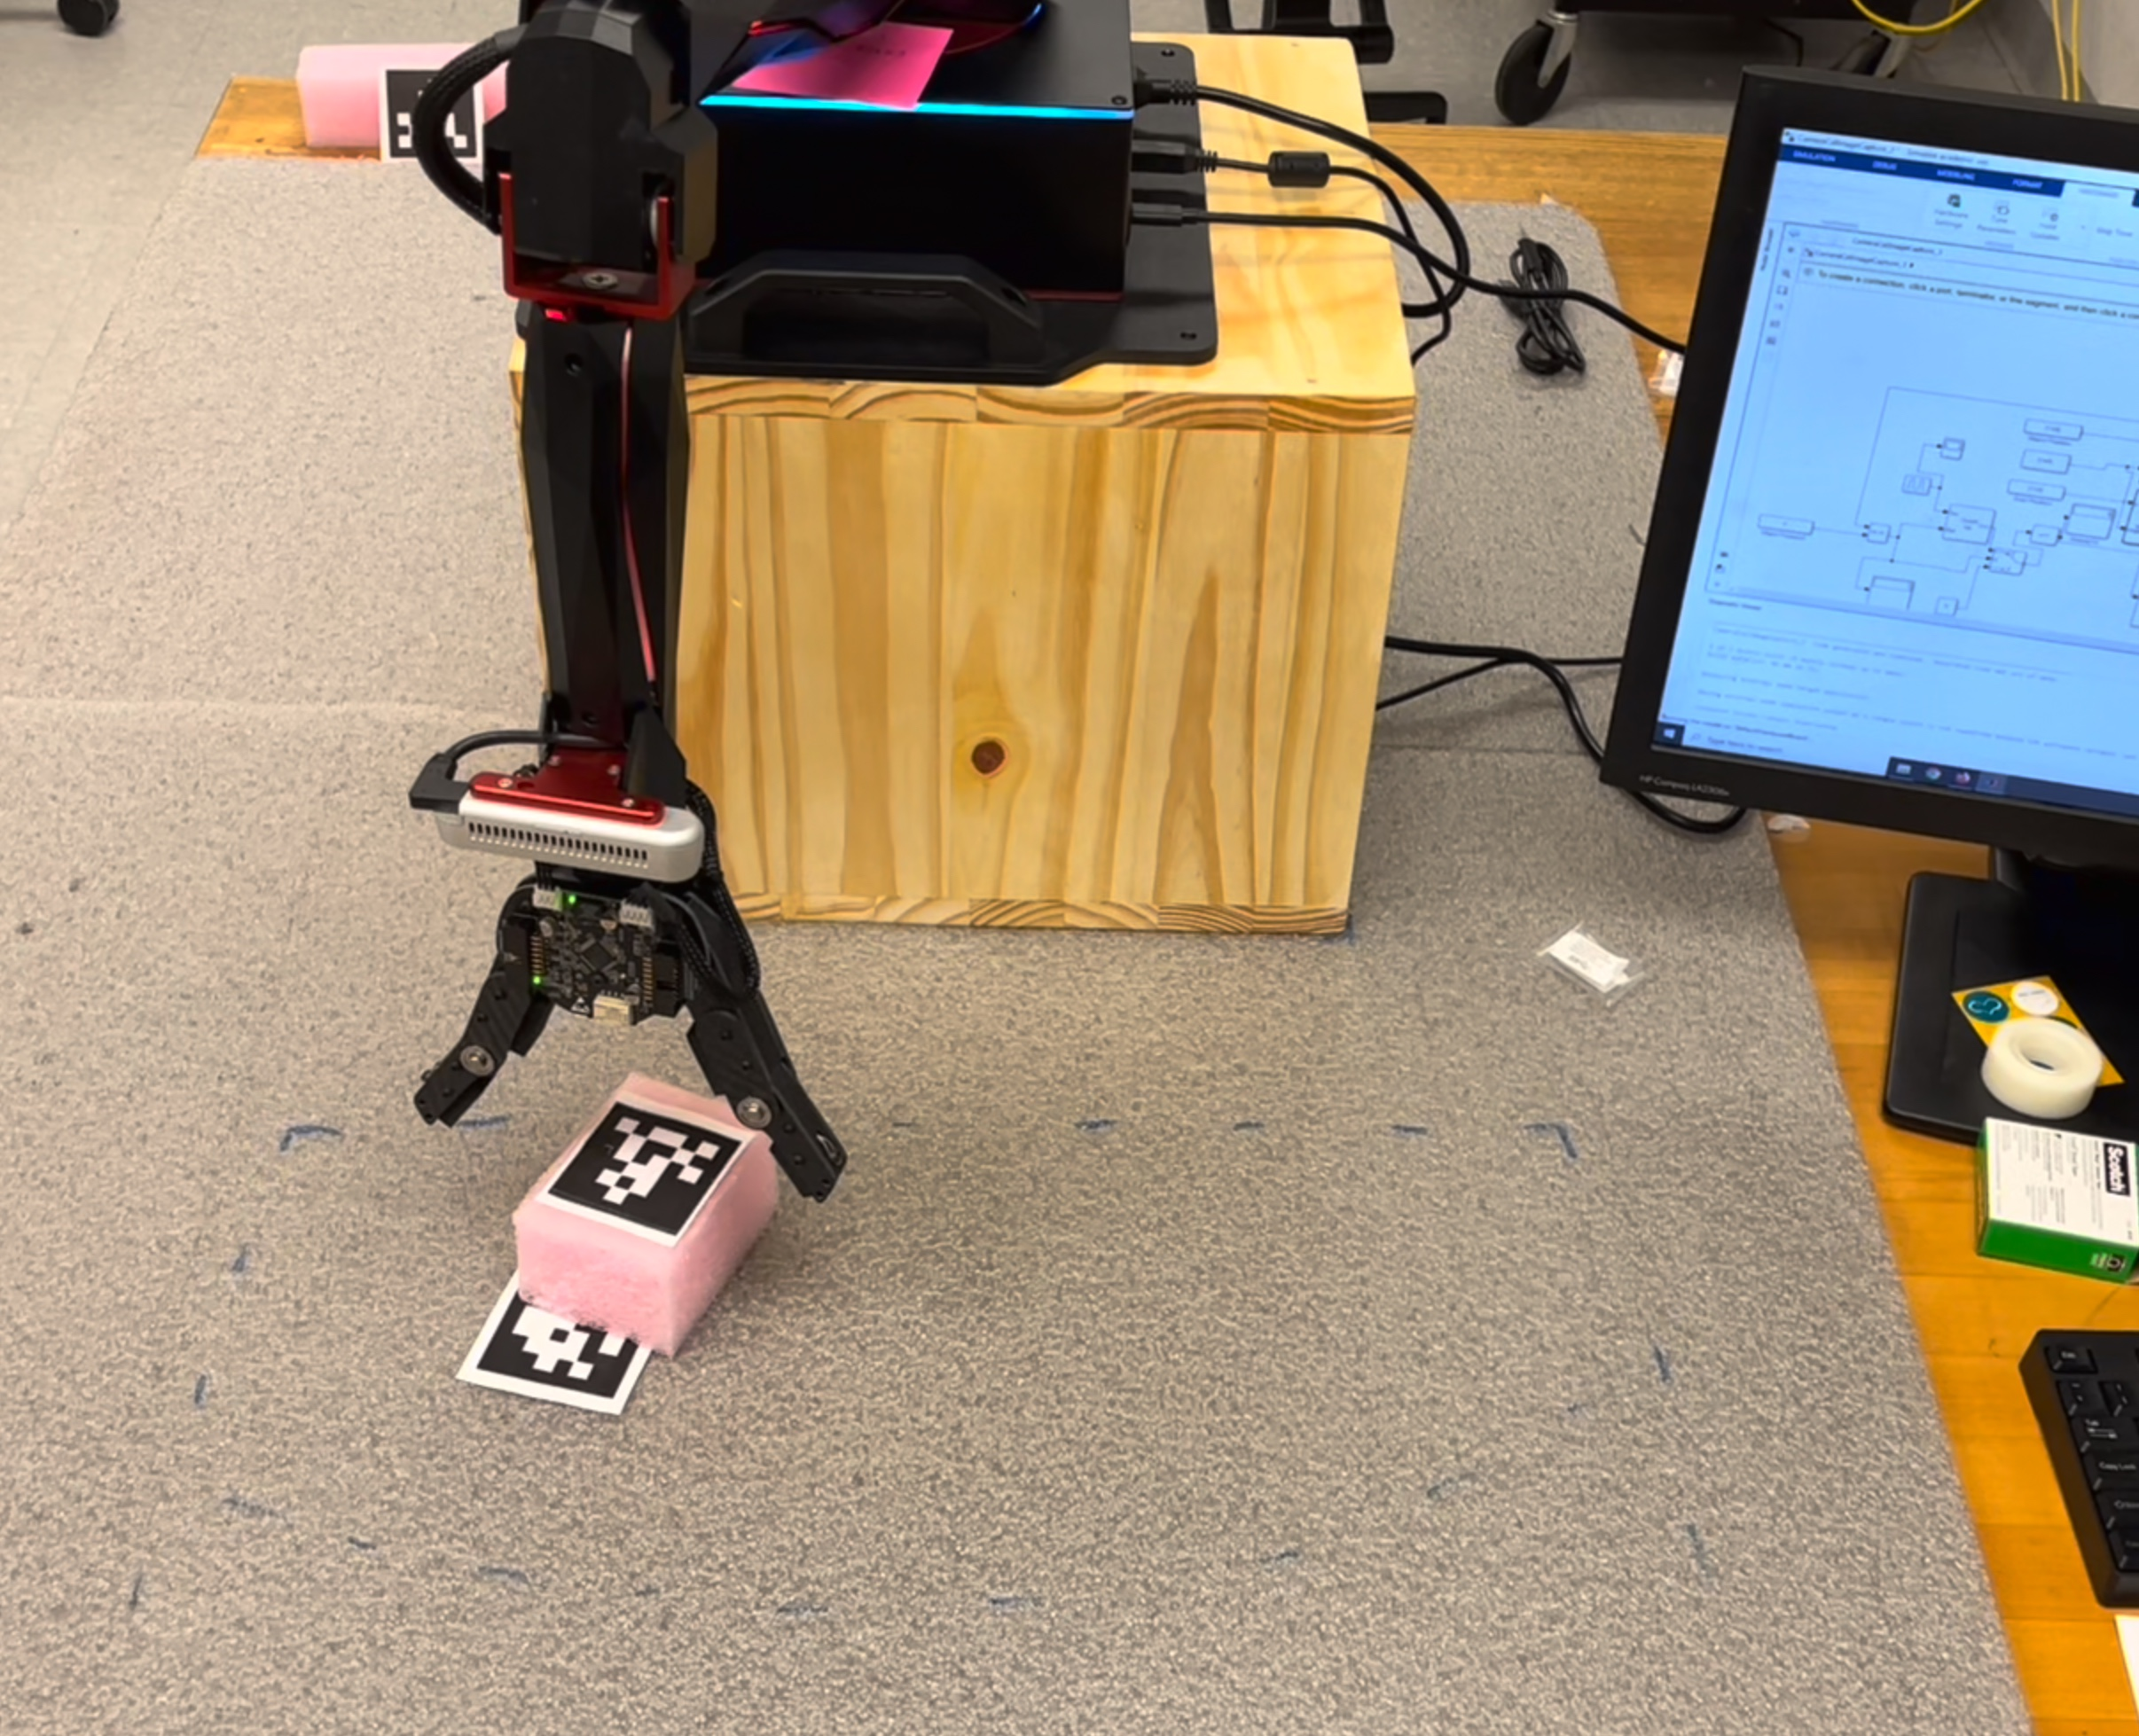
\includegraphics[width=7cm]{Figures/Drop-Off.jpeg}
\caption{Dropping off the object}
\centering
\end{figure}
